\documentclass[11pt]{beamer}
\usetheme{Rochester}
\usepackage[utf8]{inputenc}
\usepackage[french]{babel}
\usepackage[T1]{fontenc}
\usepackage{amsmath}
\usepackage{amsfonts}
\usepackage{amssymb}
\usepackage{graphicx}
\author{Fahy Axel \& Höhn Rudolf}
\title{Kohonen Network}
%\setbeamercovered{transparent} 
%\setbeamertemplate{navigation symbols}{} 
%\logo{} 
\institute{Algorithmes avancées\\hepia} 
%\date{} 
%\subject{} 
\begin{document}

\begin{frame}
\titlepage
\end{frame}

\begin{frame}
\tableofcontents
\end{frame}

\section{Structure du projet}
\begin{frame}{Structure du projet}
\begin{center}
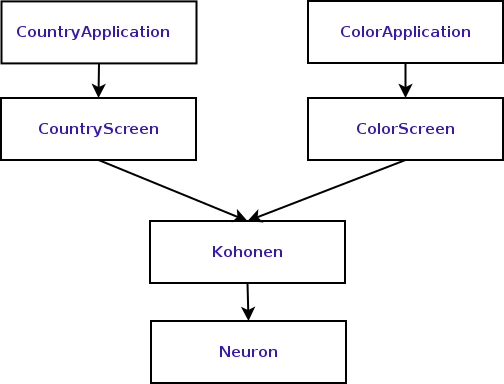
\includegraphics[scale=0.5]{KohonenDiagram.png} 
\end{center}
\end{frame}

\section{Données comparées}
\begin{frame}{Données comparées}
\begin{itemize}
\item \textbf{Couleurs} : sur la base des valeurs rouge, vert et bleu (RGB) d'un élément
\item \textbf{Pays} : sur la base du PIB et de son évolution, par habitant, entre les années 2008 et 2013
\item \textbf{Normalisation des données} : l'algorithme SOM fonctionne sur des vecteurs à composantes se situant entre $[0, 1]$
\end{itemize}
\end{frame}

\section{Résultats}
\begin{frame}{Résultat couleurs}
\begin{center}

\includegraphics[scale=0.25]{colors.png} 
\end{center}

\end{frame}

\begin{frame}{Résultat pays}

\end{frame}

\section{Démo}
\begin{frame}{Démo}
\end{frame}

\end{document}